\subsection{Elettronica di misura}

\marginpar{Stavolta Jack ci delizierà con i suoi fantastici disegni?}

I segnali analizzati in questa esperienza provengono da un fotodiodo al silicio la cui uscita è inviata ad un insieme di discriminatori e preamplificatori. Essi forniscono un segnale logico TTL ed un segnale analogico NIM preamplificato, entrambi della durata di pochi \si{\micro s}.
Disponiamo di un amplificatore che genera un segnale la cui altezza di picco è proporzionale all'energia rilasciata nel fotodiodo.
\marginpar{do per scontato che nella \emph{Teoria} sia scritto che il fotodiodo assorba tutta l'energia delle $\alpha$}
Tale picco viene letto da un'ADC a \SI{12}{bit}. Gli altri strumenti sono i soliti moduli (contatori, timer, coincidenze...) presenti in laboratorio.

\subsection{Strategia di acquisizione}

\paragraph{Angoli}
Ci accorgiamo che non siamo in grado di sistemare il coperchio della camera a vuoto esattamente nello stesso punto ogni volta che chiudiamo la camera. Eliminiamo questa sistematica sfruttando il fatto che il coperchio ha un foro che deve essere posizionato al di sopra di un perno. Dopo averlo incastrato lo spingiamo a sinistra e, una volta fatto il vuoto, la pressione atmosferica renderà impossibile spostarlo.
Questo accorgimento ci permette di riposizionare la sorgente nello stesso punto della scala graduata. Cercheremo gli angoli ``veri'' attraverso l'analisi delle nostre misure.
\marginpar{non so come spiegare questa cosa dell'angolo vero con parole migliori}
Riduciamo la parallasse nell'allineamento attaccando un pezzo di carta con una tacca al supporto della sorgente.
\marginpar{spiegare meglio il pezzo di carta (io metterei la foto senza aggiungere altro)}

\paragraph{Energia}
Per acquisire al meglio i segnali amplificati dobbiamo costruire un circuito che sincronizzi il contatore e l'ADC all'inizio e alla fine di ogni acquisizione.
Vogliamo comandare l'inizio e la fine di ogni acquisizione agendo sulla levetta di un timer.
I conteggi vengono effettuati collegando l'uscita TTL del discriminatore ad un generatore di impulsi non retriggerabile, la cui uscita va ad un contatore. Per far partire e fermare un'acquisizione elettronicamente è sufficiente collegare l'uscita del timer allo \emph{start} del contatore e l'\emph{end marker} allo \emph{stop}.
Per fare la stessa cosa con l'ADC colleghiamo l'uscita del timer (con durata impostata su $\infty$) ad un modulo di coincidenze a cui è connessa, ad un altro ingresso, l'uscita TTL del generatore di impulsi convertita in NIM. Il segnale di coincidenza (convertito in TTL) sarà il trigger dell'ADC, che deve arrivare all'omonimo ingresso \SI{1}{\micro s} prima del segnale affinché ne selezioni il picco.
Concludiamo la procedura inserendo i ritardi opportuni.

\paragraph{Precauzioni}
Evitiamo che segnali superiori a \SI{3.3}{V} danneggino l'ADC ponendo un attenuatore da \SI{0.9}{dB} all'uscita dell'amplificatore. Per il trigger non è necessario prendere precauzioni in quanto il convertitore NIM-TTL fornisce un segnale della tensione giusta. \marginpar{misurare?}


\subsubsection{Taratura ADC}
L'ADC è stata tarata ponendo la sorgente a \SI{0}{\degree} e variando il ritardo sul trigger fino a massimizzare la lettura del segnale. Il risultato di tale misura è presente in \autoref{tara}. Abbiamo acquisito lo spettro a vari angoli e verificato che l'energia delle particelle $\alpha$ non dipendesse dall'angolo in assenza di bersaglio. 
\marginpar{il fit e la figura sono degli scalda posto per sapere come verrà in seguito}
Abbiamo fittato lo spettro a \SI{0}{\degree} con una Gaussiana lasciandone libera anche la normalizzazione.\\
Abbiamo ottenuto:
\begin{align*}
\mu &=3115\pm2 \\
\sigma &= 87\pm2 \\
N &=(1.18\pm0.02)\cdot10^5 \\
\chi^2 &=2313\pm15 \\
\text{dof} &=15 \\
\end{align*}
Il valore elevato del $\chi^2$ mostra chiaramente la non gaussianità del picco osservato.

\begin{figure}[h]
\centering
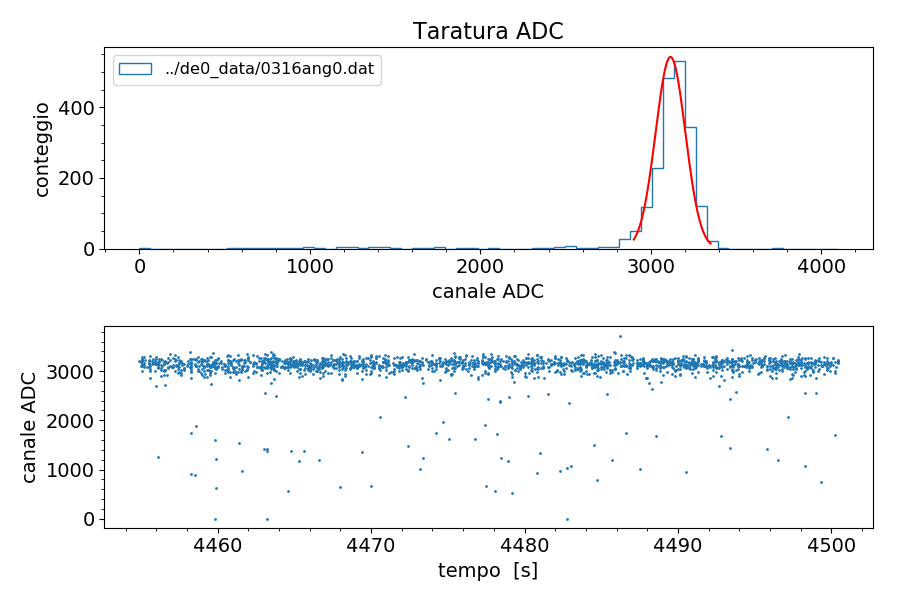
\includegraphics[width=23 em]{immagini/cal_provv}
\caption{Risoluzione in energia dell'ADC. Il pannello superiore mostra l'istogramma dei dati acquisiti con la funzione di fit, quello inferiore mostra il loro valore in funzione del tempo.}
\label{tara}
\end{figure}